% 222.jpg
\begin{exercises}

\exercise 一轻弹簧垂直悬挂,下端挂上一个质量$ m _ 1 $为$ 2.0 $千克的物
体,然后再挂上一个质量$ m _ 2 $为$ 300 $克的物体,测得弹簧又拉长了
$ 2.0 $厘米。如将$ m _ 2 $取下,而使$  m _ { 1 } $振动,求振动周期$ T $。

\exercise 用等长的两根不可伸长的细线挂在同一悬点的两个小球,
质量分别为$ m $和$ 2m $,将它们分别向左右拉开一个不太大的角位移
$ \theta _ { 1 } $和$ \theta _ { 2 } $,同时由静止自由摆下。试问:它们将在什么地方相碰?

\exercise 比较$ x _ { 1 } = A _ { 1 } \cos \left( \omega t + \uppi / 2 \right) $与$ x _ { 2 } = - A _ { 2 } \sin \omega t $之间的位相
关系。

\exercise 将单摆从平衡位置拉开一个很小的角度$ \varphi $,然后放手任其
摆动,并开始计时。试问:此$ \varphi $角是否就是单摆作简谐振动的初
位相?如果不是,那么单摆作简谐振动的初位相$ \varphi _ { 0 } $是多少?

\exercise 某一质点按下列规律运动:
\begin{equation*}
    y = A \sin \omega t + B \sin 2 \omega t
\end{equation*}
其中$ A $,$ B $,都是常数。试问:

(1)速度、加速度、将遵守什么规律?

(2)是简谐运动吗?

\exercise (1)试证:任一简谐运动的周期和频率的公式是
\begin{equation*}
    T = 2 \uppi \sqrt { - \frac { x } { \ddot { x } } } , \quad v = \frac { 1 } { 2 \uppi } \sqrt { - \frac { \ddot { x } } { x } }
\end{equation*}

(2)试证:任一角简谐运动的周期和频率的公式是
\begin{equation*}
    T = 2 \uppi \sqrt { - \frac { \theta } { \ddot { \theta } } } , \quad v = \frac { 1 } { 2 \uppi } \sqrt { - \frac { \ddot { \theta } } { \theta } }
\end{equation*}

\exercise 把一质量为$ m $的物体挂在吊着的轻弹簧下端,静止后弹簧
伸长了$ l $,随后让此系统自由振动。试证:这系统的振动周期与一
长为$ l $的单摆的周期相同。

% 223.jpg
\exercise 把一重物挂在吊着的轻弹簧下端,静止后弹簧伸长$ l = 10 $
厘米;再把重物往下拉一段距离$ d = 2.0 $ 厘米,并在位移方向给它
一个初速度$ v _ { 0 } = 10 $厘米/秒,然后放手任其自由振动。不计空气阻
力,试求:

\begin{wrapfigure}[7]{r}{9em}
    \vspace{-1.56em}
    \centering
    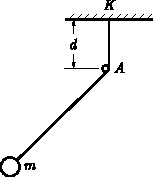
\includegraphics{figure/fig07.15}
    \caption{}
    \label{fig:07.15}
\end{wrapfigure}
(1)振动频率$ \nu $;

(2)振幅$ A $;

(3)初位相$ \varphi _ { 0 } $;

(4)振动的数学表达式。

\exercise 如图\ref{fig:07.15},摆长$ l = 150 $厘米,在顶
点$ K $的正下方距$ K $为$ d = 54 $厘米处有一钉
子$ A $,求这摆的周期$ T $。

\exercise 一物体作简谐振动,在什么时候动能与位能相等?

\exercise 质量为$ m = 121 $克的水银装在U形管中,管的横截面积为
$ S = 0.3 \text { 厘米 } ^ { 2 }$,水银的密度$ \rho = 13.6 \text { 克 } / \text { 厘米 } ^ { 3 }$,向U形管的一端吹气,
使另一端的水银面升高,然后让水银在管内自由振动。求振动的
周期$ T $。

\exercise 将一质量$ m $系于竖直悬挂的弹簧的下端,弹簧的端点以
$ 2.0 $秒的周期振动。将这个质量再增加$ 2.0 $千克,周期就变为$ 3.0 $
秒。试求$ m $。

\exercise 一物体放在一活塞上,活塞在竖直方向作简谐运动,其
周期为$ 1 $秒。问:

(1)在多大振幅时,物体与活寒将相互分离?

(2)如果活塞具有$ 5.0 $厘米的振幅,物体与活塞保持接触的最
大频率为多大?

\exercise 一物体放在一水平面上,水平面以$ 2 $赫兹的频率作水平简
谐运动。物体和平面之间的静摩擦系数为$ 0.50 $。试问:如果物体
不沿着水平面滑动,它的最大振幅是多少?

\exercise 两质点沿着同一直线作相同频率和相同振幅的简谐运
% 224.jpg
动。若它们每次沿相反方向相互通过时,它们的位移均为各自振
幅的一半,试问:它们的相差是多少?

\exercise 将一倔强系数$ k = 7.0 $牛顿/米、无质量的弹簧切成相等的
两段,试问:

(1)每一段的倔强系数是多少?

(2)将这两段并联吊着一个质量为$ M $的重物,若这个振动系
统的自由振动频率为$ 3.0 $赫兹,$ M $是多少?

\exercise 一均匀无质量的弹簧,它的长为$ l $,倔强系数为$ k _ { 0 } $将这弹l
簧切成自然长度为$ l _ { 1 } $及$ l _ { 2 } $的两段,且$ l _ { 1 } = n l _ { 2 } $($ n $为一个整数)。试用
$ n $,$ k $表示相应的倔强系数$ k _ { 1 } $,$ k _ { 2 } $。

\begin{wrapfigure}[4]{r}{17em}
    \centering
    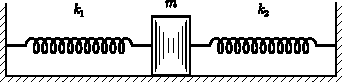
\includegraphics{figure/fig07.16}
    \caption{}
    \label{fig:07.16}
\end{wrapfigure}
\exercise 如图\ref{fig:07.16}\;所示,将$ m $连接在两个弹
簧$ k _ { 1 } $,$ k _ { 2 } $ 之间。试问:这
系统的振动频率$ \mu $是什么?(不计摩擦及弹簧的质量。)

\exercise 一不计质量、自然长度为$ l $的弹簧,两端分别系上质量为
$ m _ { 1 } $和$ m _ { 2 } $的小物体,并放在光滑的水平桌面上(图\ref{fig:07.17})。手持$ m _ { 1 } $和$ m _ { 2 } $把弹簧拉长为$ l' $,停止不动,然后放手。求这系统的运动。
\begin{figurex}
    \centering
    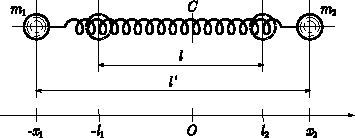
\includegraphics{figure/fig07.17}
    \caption{}
    \label{fig:07.17}
\end{figurex}

\exercise 弹簧及两物体连接如图\ref{fig:07.18}\;所示。将$ m _ 1 $拿在手上,$ m _ 2 $自
由下垂,
垂,待静止后放手。求物体的运动。

\exercise 一摆由很轻的棒和固定在它两端的相同的重物$ m $做成一
% 225.jpg
\begin{figurex}
    \begin{minipage}[b]{0.5\linewidth}
        \centering
        
\includegraphics{figure/fig07.18}
        \caption{}
        \label{fig:07.18}
    \end{minipage}
    \begin{minipage}[b]{0.5\linewidth}
        \centering
        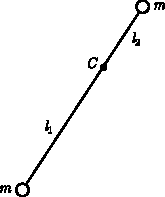
\includegraphics{figure/fig07.19}
        \caption{}
        \label{fig:07.19}
    \end{minipage}
\end{figurex}
个重物到转轴$ C $的距离$ l _ { 1 } = 30 $厘米,另一个$ l _ { 2 } = 15 $厘米(图\ref{fig:07.19})
试求:

(1)它作微小振动时的周期$ T $;

(2)它的折合摆长$ l _ { 0 } $,即把它看成一个单摆时的等效摆长。

\exercise 若沿地球直径凿一条隧道,并设地球密度$ \rho = 5.5 \text { 克 } / \text { 厘米 } ^ { 3 } $
的均匀球体。试证:

(1)当无阻力时,一物体落入此隧道后将作简谐运动;

(2)由地球表面落至地心的时间为
\begin{equation*}
    t = \frac { 1 } { 4 } \sqrt { \frac { 3 \uppi } { G \rho } } = 21 \text { 分 }
\end{equation*}
式中$ G $是引力常数。

\exercise 火车在铁轨上行驶,每经过接轨处即受一震动,使车厢在
弹簧上面上下振动。设每段铁轨长$ 12.5 $米,弹簧平均负重$ 5.5 $吨,
而弹簧每受$ 1 $吨力将压缩$ 16 $毫米。试问:火车速度多大时,振动
特别强?

\exercise 有一音叉,在$ 440 $赫兹时发声,声平计指出,声音强度在
$ 4.0 $秒之内减小到$ 1/5 $。试求音叉的$ Q $值。

\exercise 将一根橡皮带悬挂起来,测得它的振动周期为$ 1.2 $秒,$ 3 $个
周期后,振幅减小到$ 1/2 $。试估计这个系统的$  $Q值。


\end{exercises}